\chapter{Informality and Labour Markets in Developing Countries}

\fancyhead[L]{ECON0024}
\fancyhead[C]{Ch.6 Informality and Labour Markets}
\fancyhead[R]{Xiaotian Tian}
\fancyfoot[L]{\hyperlink{tableofcontents}{Back to Table of Contents}}
\fancyfoot[R]{Xiaotian Tian}

\section{Basics and Facts: Unemployment, Informality, and Frictions in Labour Markets of Developing Countries}

    \subsection{Unemployment and Informality}
    
        \subsubsection{Unemployment is Not a "Rich Countries' Problem"}
            Evidences show that unemployment is even a bigger issue for poor countries:
            \begin{figure}[H]
                \centering
                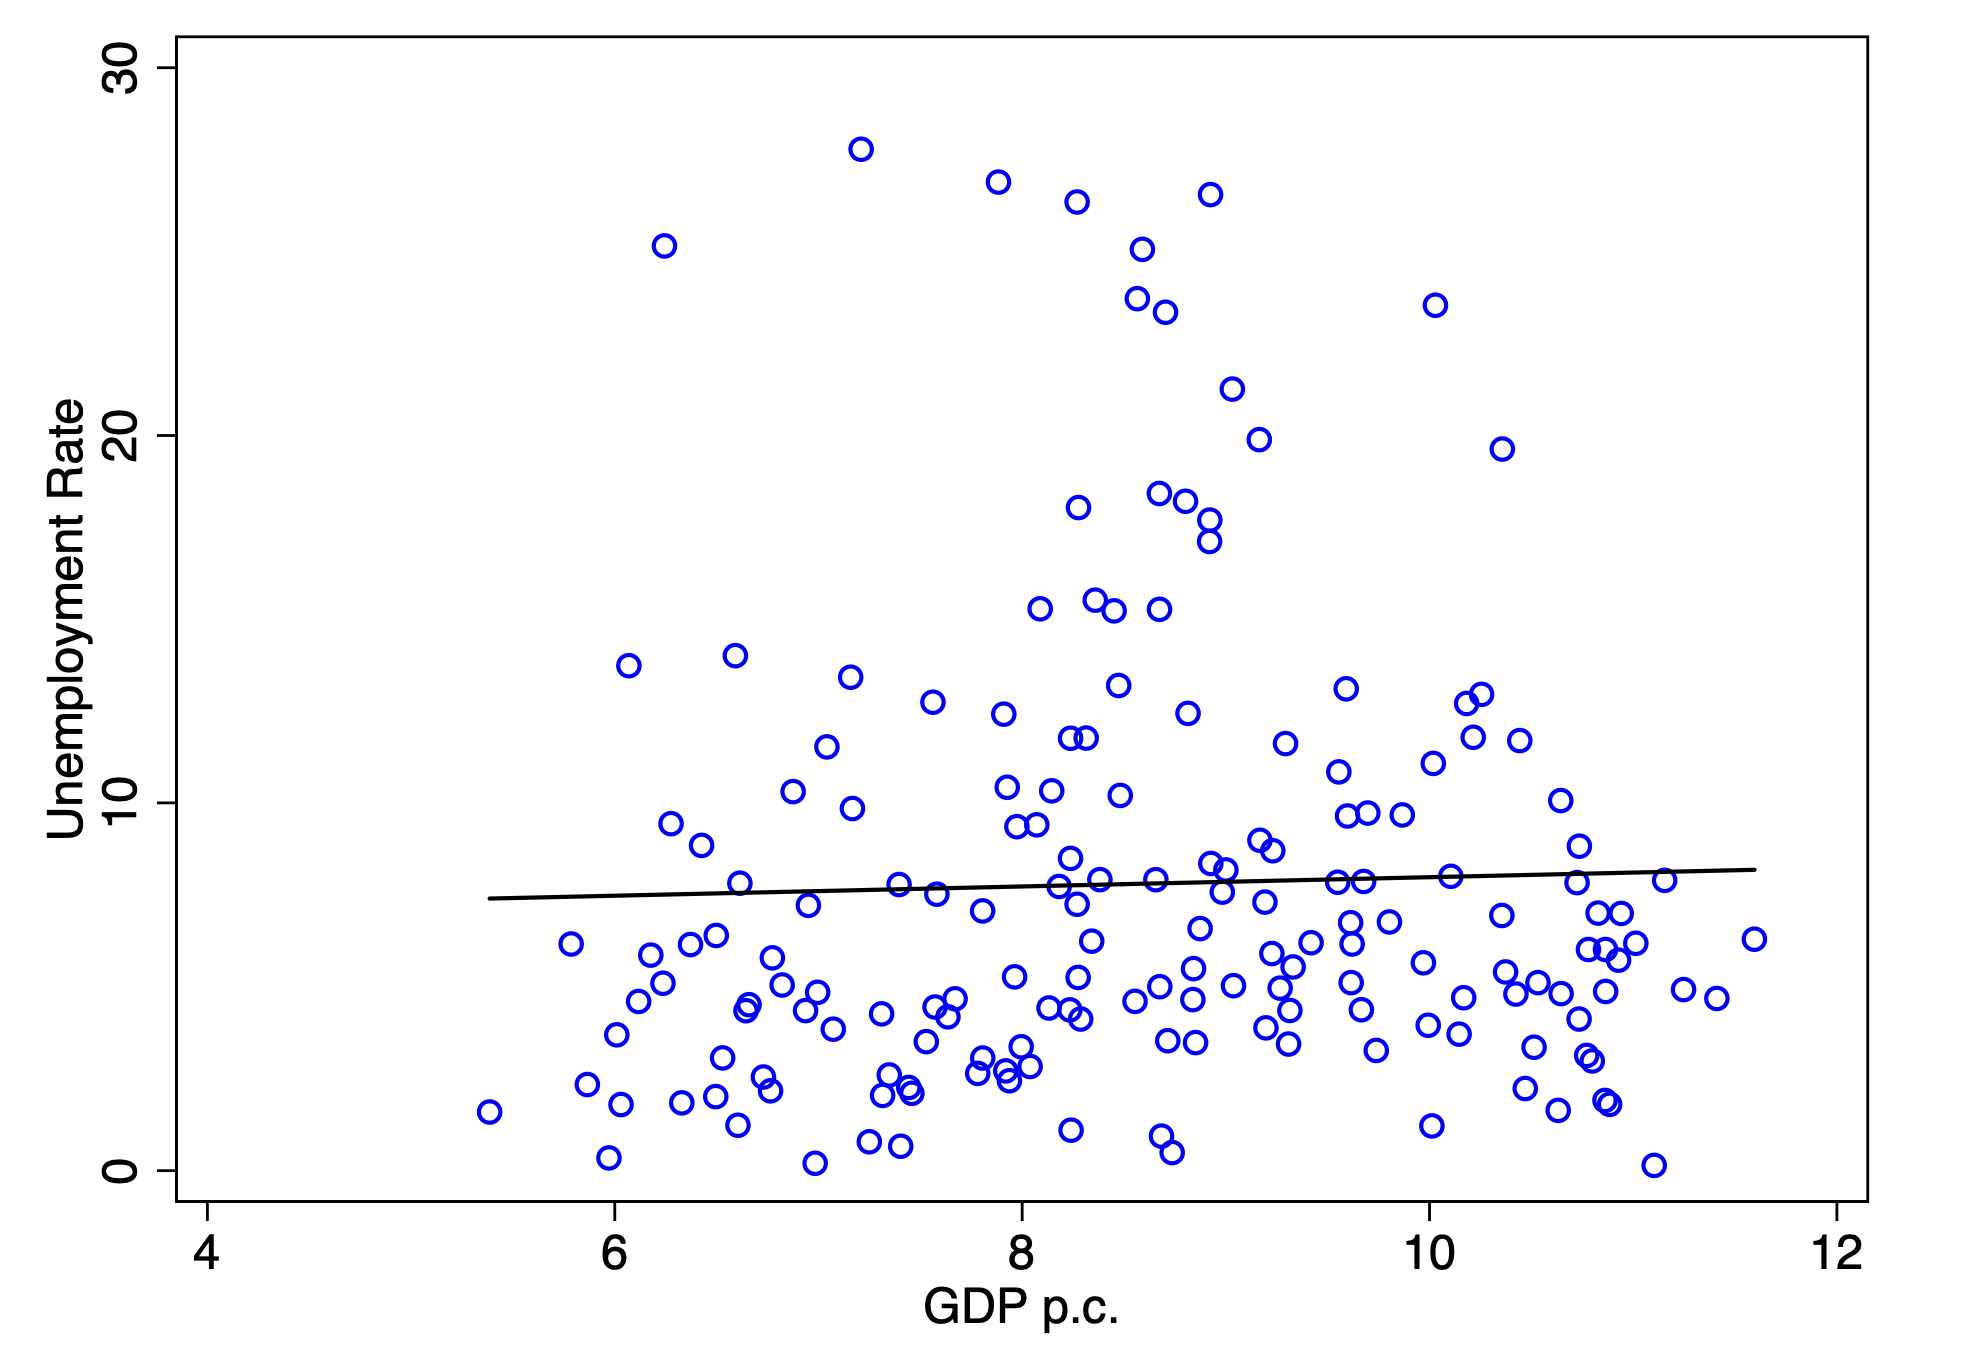
\includegraphics[width=2.75in]{images/ch6/unemp_gdp_1.png}
                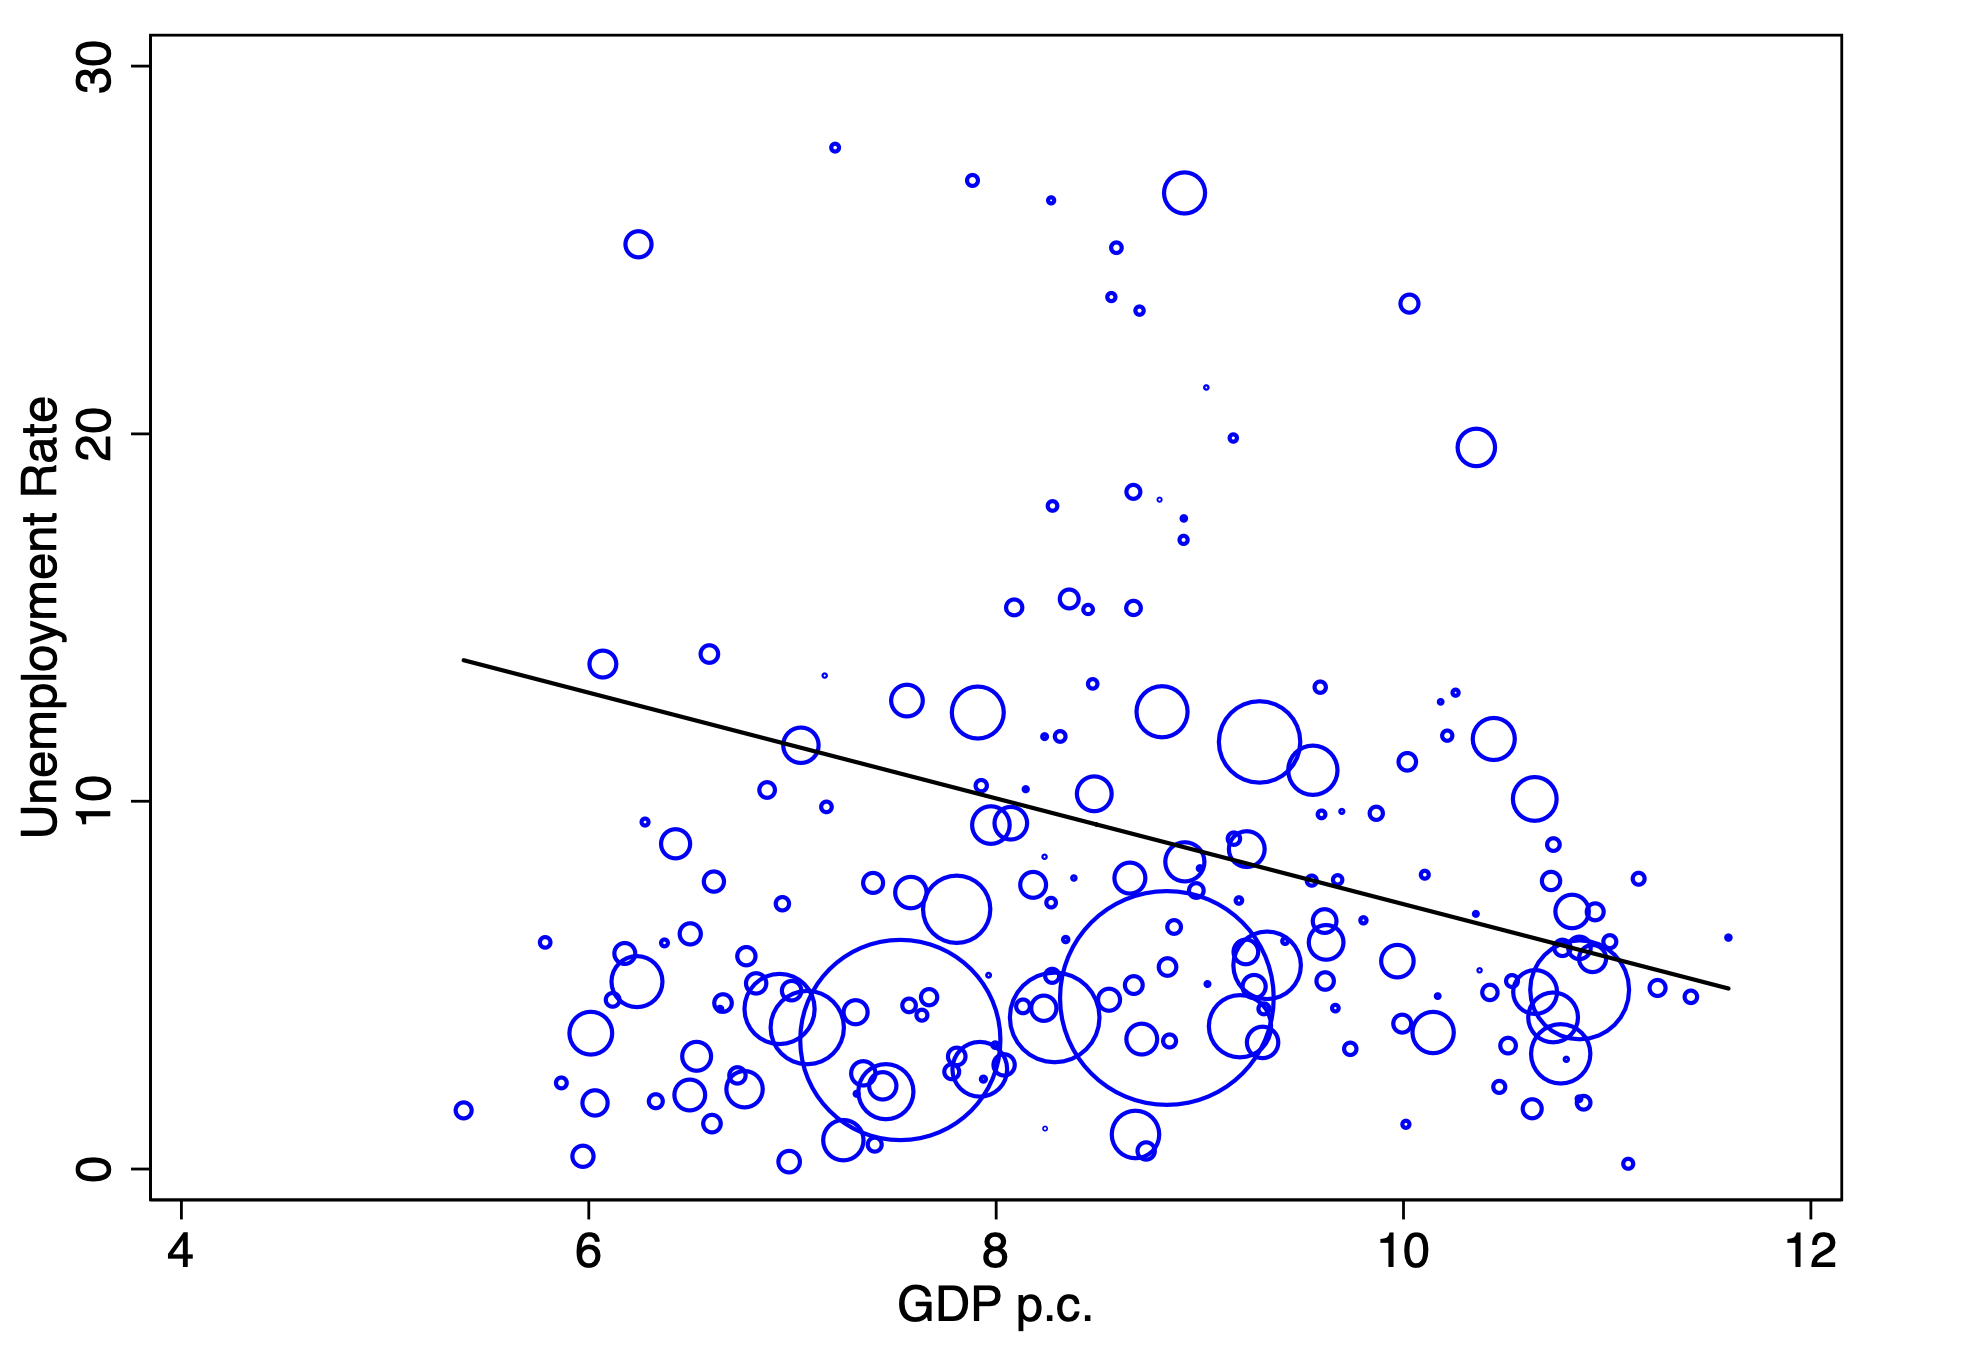
\includegraphics[width=2.75in]{images/ch6/unemp_gdp_2.png}
                \caption{Unemployment Rate and GDP per Capita (L: Equal Weight; R: Weighted by Population) (\cite{the_world_bank_world_2022})}
            \end{figure}
            
        \subsubsection{Informality and Employment: Issues \& Benefits}
            \begin{figure}[H]
                \centering
                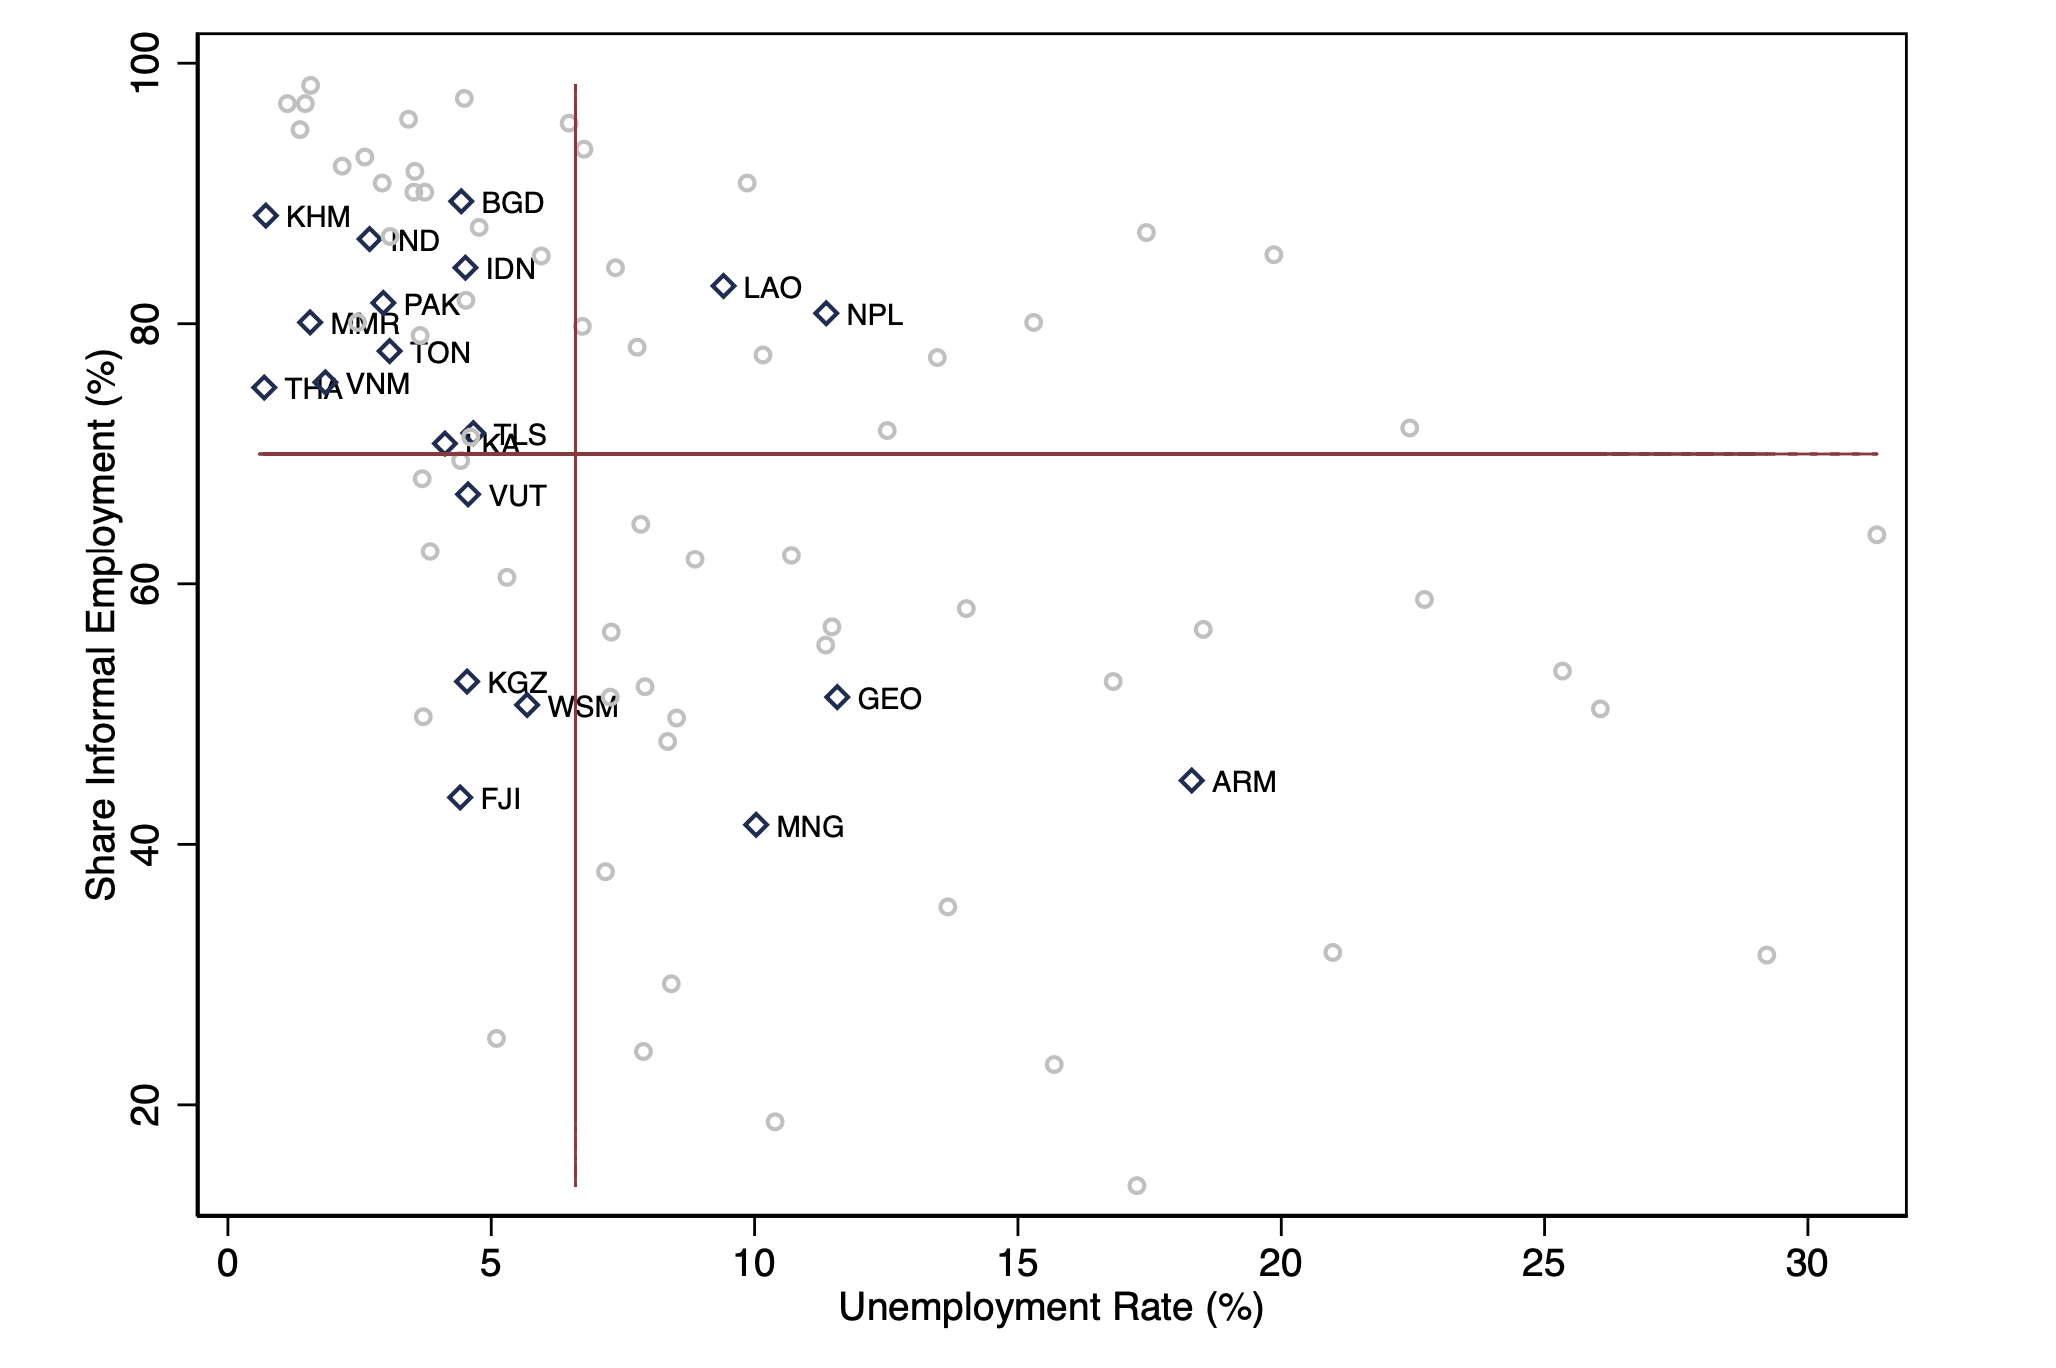
\includegraphics[width=4in]{images/ch6/informal r unemployment r.png}
                \caption{Share of Informal Employment and Unemployment Rate}
            \end{figure}
            Informality is clearly more common for developing countries, and there is an equilibrium of low unemployment and high informality, indicated by the figure above.
            \begin{figure}[H]
                \centering
                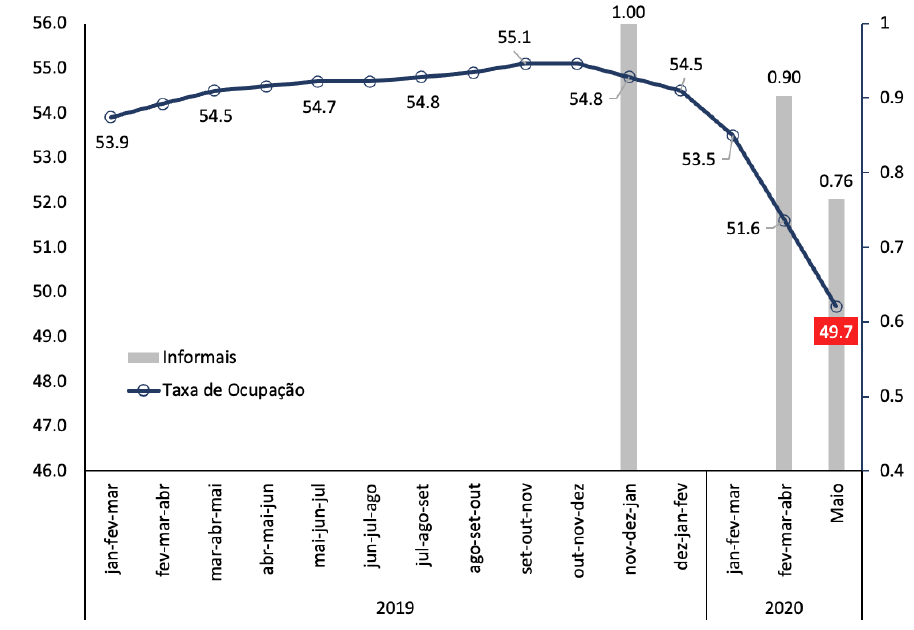
\includegraphics[width=4in]{images/ch6/informal emp during crisis.png}
                \caption{Overall Employment and Informal Employment during Crisis}
            \end{figure}
            During crisis, high informality could be a problem as there's \emphb{no firing cost} to layoff informal workers. This is observed during Covid in Brazil: while the overall unemployment dropped by 6\%, informal employment decreased for around 25\%.
            \begin{figure}[H]
                \centering
                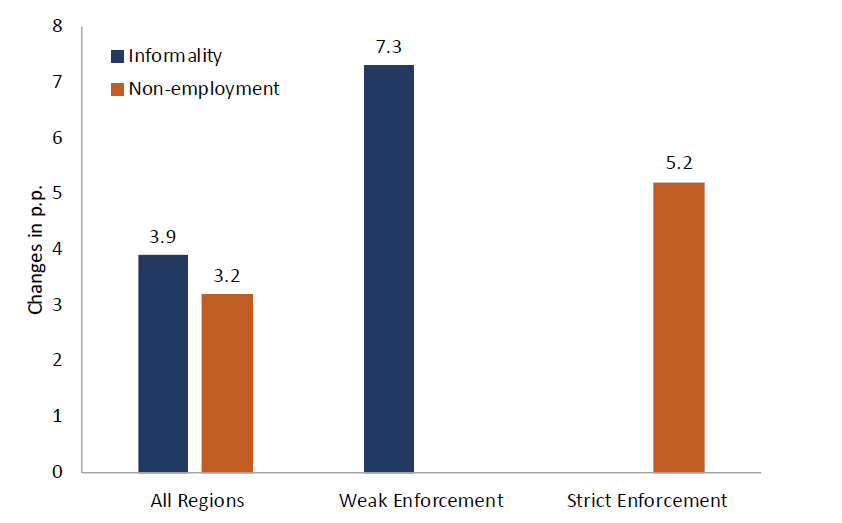
\includegraphics[width=4in]{images/ch6/employment brazil 1990 lib.png}
                \caption{Dynamics of Formal/Informal Employment during Brazil's 1990 Trade Liberalisation (\cite{ponczek_enforcement_2022})}
            \end{figure}
            However, on the other hand, informal employment could be an \emphb{employment buffer} when the economy is facing some shocks. The figure above shows the dynamics of employment after Brazil's 1990 trade liberalisation, an unilateral trade openness reform which introduced strong competition from imports. In regions with weak enforcement, we witness an upsurge in informal employment while no change in non-employment, indicating a massive transfer from formal to informal sector. In regions with strict enforcement, there is no increase in informality, but tremendous non-employment.
            \begin{figure}[H]
                \centering
                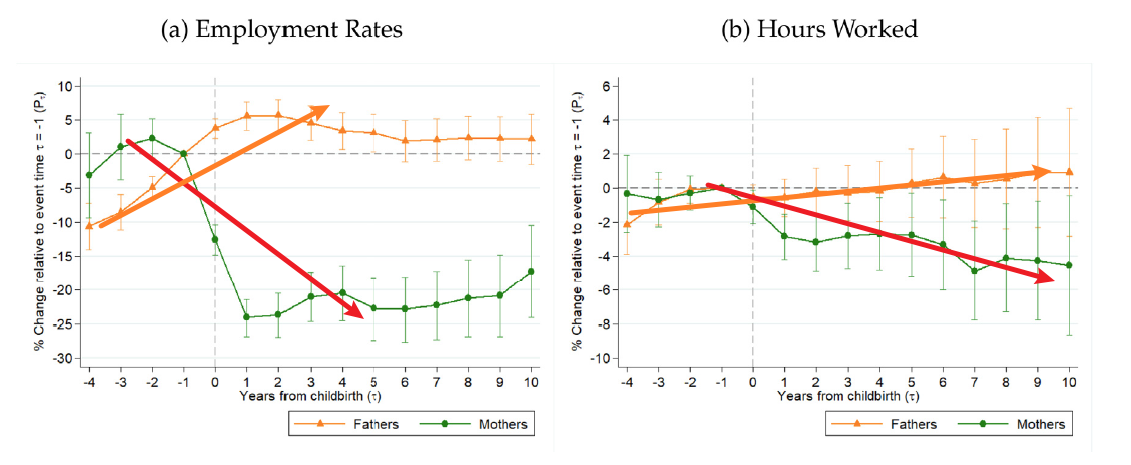
\includegraphics[width=5.5in]{images/ch6/child cost of females.png}
                \caption{Child Cost of Females}
            \end{figure}
            Informality may also provides some \emphb{flexibility to workers}. Researchers found significant "child costs" for females: after the birth of the first child, employment indicators of fathers show no sign of deterioration while those of mothers slump. This could be caused by the uneven distribution of caring responsibilities due to social norms. With more time devoted to childcare, it becomes hard for mothers to find formal jobs, and informal employment, with more flexibility, could be an alternative as indicated below:
            \begin{figure}[H]
                \centering
                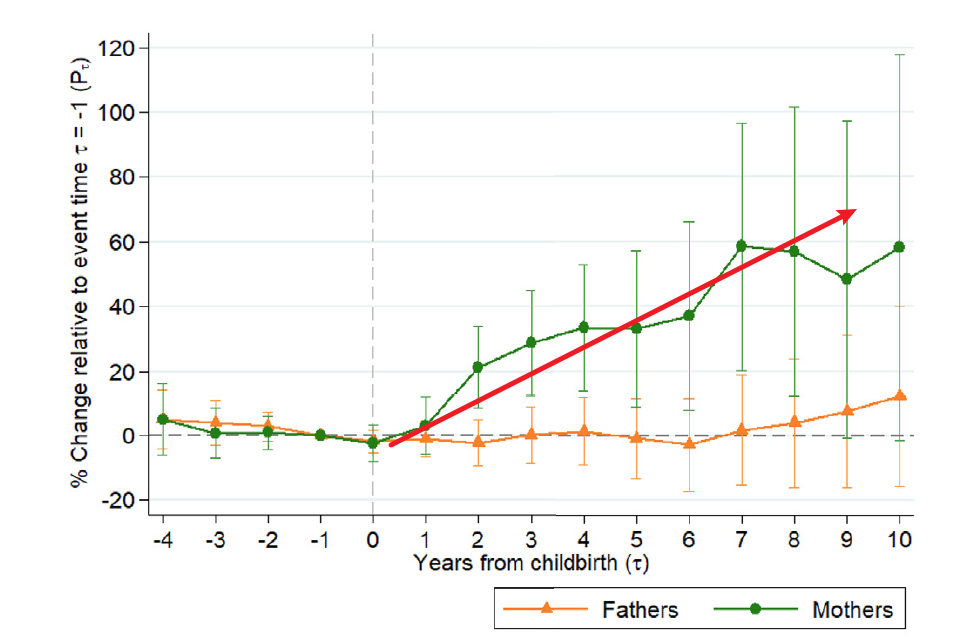
\includegraphics[width=4in]{images/ch6/child cost and informality.png}
                \caption{Child Birth and Informality}
            \end{figure}
            One caveat: the overall welfare effects are ambiguous and \empha{always depend on the counterfactual}.
            
    \subsection{Labour Market Frictions}
        \emphb{Labour Market Frictions} include imperfect information, dispersion of workers and jobs across space (spatial immobility), mobility costs, cultural factors, uncertainty, etc.
        
        \subsubsection{Social Network: an Indicator of Information Efficiency}
            \begin{figure}[H]
                \centering
                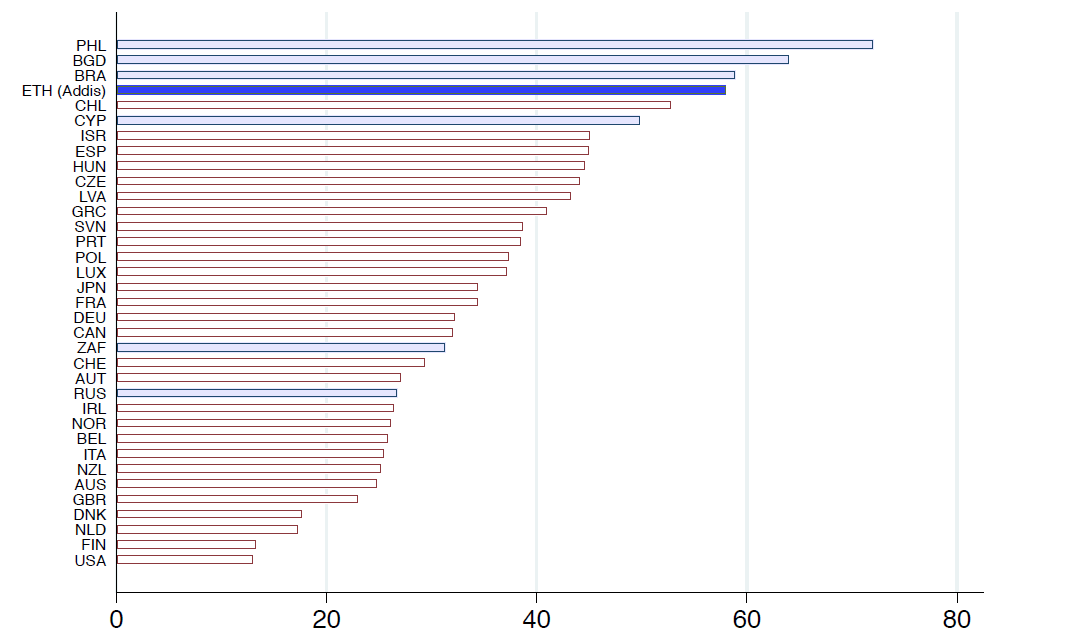
\includegraphics[width=4in]{images/ch6/social networks.png}
                \caption{Heard of Current Job from Social Networks (\%) (\cite{witte_job_2018})}
            \end{figure}
            The figure above shows the proportion of employed individuals heard of their current jobs from \emphb{social networks}. This measure the importance of social network in an economy's labour market. Typically, higher shares indicate poor alternatives to gather information.
            \begin{figure}[H]
                \centering
                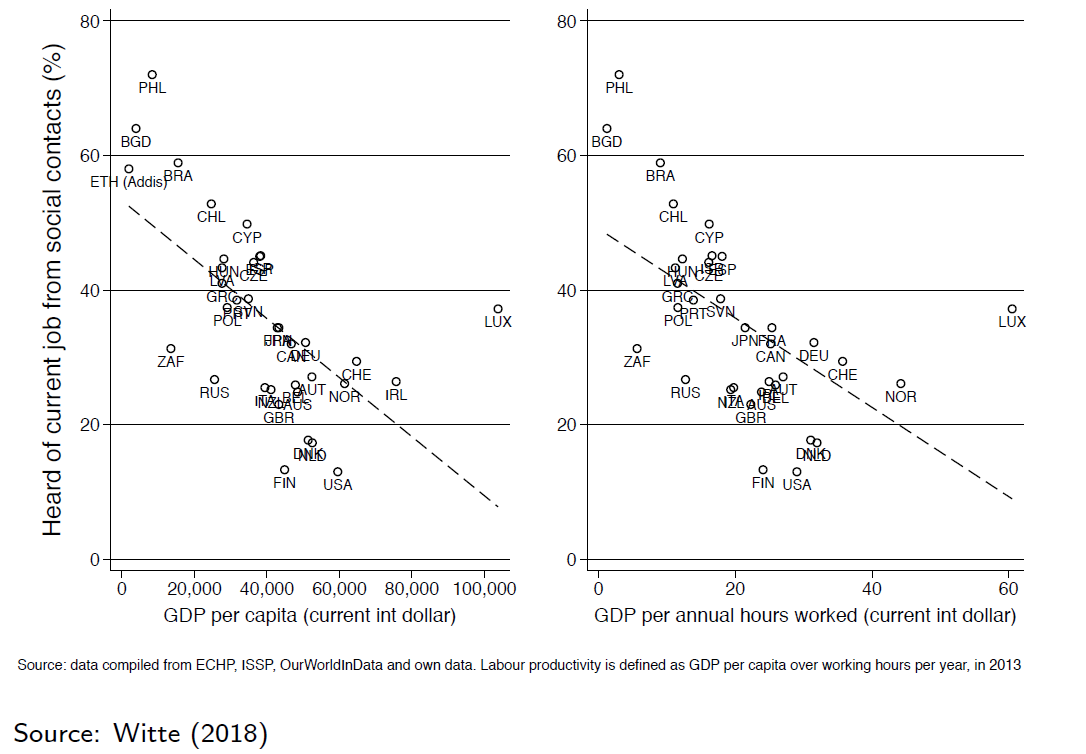
\includegraphics[width=5in]{images/ch6/social networks and gdp per capita.png}
                \caption{Heard of Current Job from Social Networks (\%) and GDP per Capita (\cite{witte_job_2018})}
            \end{figure}
            Also, it turns out that there is a negative relationship between shares of employment heard from social networks and GDP per capita. Thus, frictions may be an important problem especially for developing countries.
            
    \subsubsection{Spatial Frictions}
        \begin{figure}[H]
                \centering
                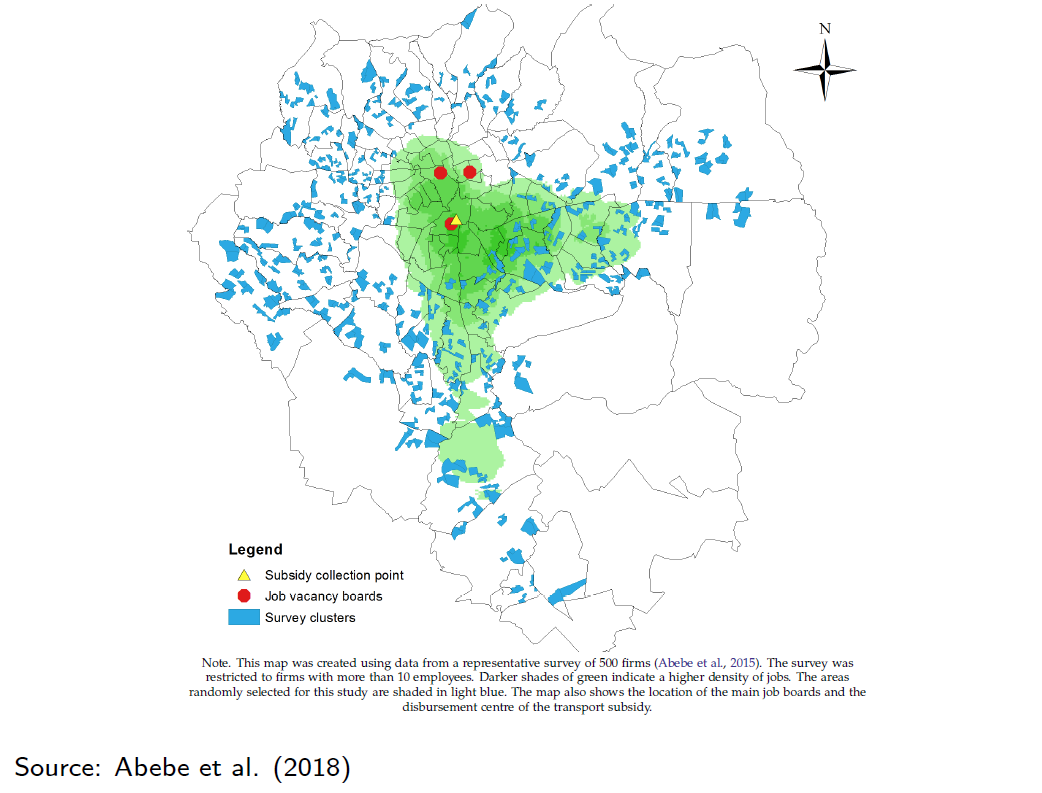
\includegraphics[width=5in]{images/ch6/spatial friction addis ababa.png}
                \caption{Spatial Frictions in Addis Ababa (\cite{abebe_anonymity_2021})}
                \label{fig:addis ababa spatial frictions}
        \end{figure}
        The blue area represent living places and green area represent job locations. Red dots are job vacancy boards where people find employment information. We can see a clear spatial mismatch between jobs, workers, and information sources.
        \begin{figure}[H]
                \centering
                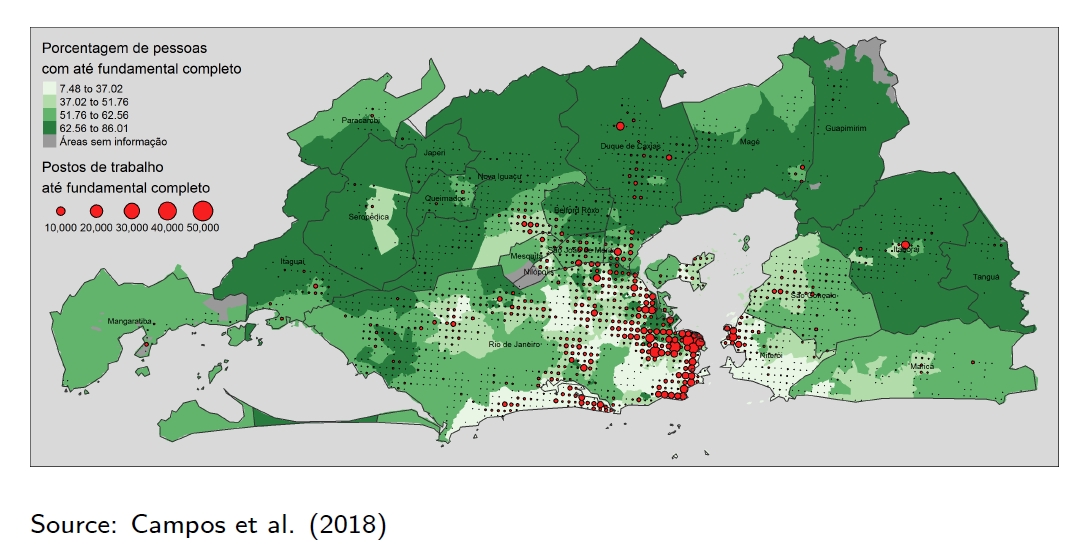
\includegraphics[width=5in]{images/ch6/spatial friction rio de janeiro.png}
                \caption{Spatial Frictions in Rio de Janeiro}
        \end{figure}
        Similar spatial frictions are observed in Rio de Janeiro: areas shaded green are places where low-skilled workers live, and red dots show formal job opportunities for those worker. Red dots are clustered around cities while workers live in rural areas.
        
\section{An Empirical Study by \cite{abebe_anonymity_2021}: Transport Subsidy and Job Application Workshop}

    \subsection{Motivation and Context}
    
        \subsubsection{Motivations}
            The youth typically work less, have lower wages, and face more job insecurities than older workers. This issue is even more severe in developing countries. Besides, lack of access to jobs among young adults is a potentially major source of inefficiency and inequality.\par
            Two main determinants of this lack of jobs:
            \begin{itemize}
                \item \emphb{High Search Costs} due to geographic dispersion, lack of information about vacancies, etc.
                \item \emphb{Information Asymmetry} between employers and workers
            \end{itemize}\par
            Abebe et al. use two treatments (transport subsidy and job application workshop) to evaluate those two causes and corresponding policies to address them.
            
        \subsubsection{Empirical Context: Addis Ababa}
             \begin{itemize}
                 \item Informal and temporary works are very common
                 \item High turnover: 72\% of jobs end within the first 3 months
                 \item Low wage growth even during periods with high economic growth
                 \item The most popular job search method is visiting job vacancy boards
                 \item Visiting vacancy boards is costly due to long travelling distance (as shown by figure \ref{fig:addis ababa spatial frictions})
             \end{itemize}
        
    \subsection{Treatments}
    
        \subsubsection{Treatment 1: Job Application Workshop}
            Job application workshops are designed to improve job-seekers' ability to present their skills accurately to potential employers (i.e. overcome anonymity). This aims to \emph{tackle with the information asymmetry} between job-seekers and employers.\par
            A workshop incorporates an orientation session and a evaluation session with certifications explaining the nature of the tests and reporting relative grades.\par
            The cost per person is 35 USD including fixed costs related to the development of tests. Excluding fixed costs, it costs only 18.2 USD per person.
            
        \subsubsection{Treatment 2: Transport Subsidy}
            Subsidies are given to individuals with an amount that can cover the cost of a return bus fare from participants' area of residence to the disbursement point (where there are job boards). This aims to reduce the cost of travelling to the city centre to gather job vacancy information and visit firms, hence \emph{reduces search costs}.\par
            The cost per person is 19.8 USD incuding all relevant costs.
            
    \subsection{Sample and Data Collection}
    
        \subsubsection{Sampling Strategy}
            Sampled areas are randomly selected geographic clusters, excluding clusters that are within 2.5km from the city centre. Then researchers use door-to-door sampling to construct a list of all individuals who:
            \begin{itemize}
                \item are between 18-29 years old
                \item completed high school
                \item are available to start working in the next 3 months
                \item don't have a permanent job or enrolled in full-time education
            \end{itemize}
            Then individuals are randomly sampled from this list with a higher frequency of from groups with higher educations.
            
        \subsubsection{Sample Balancing}
            \emph{Samples are well-balanced}: there are no significant differences between the treatment and control groups ex ante.:
            \begin{figure}[H]
                \centering
                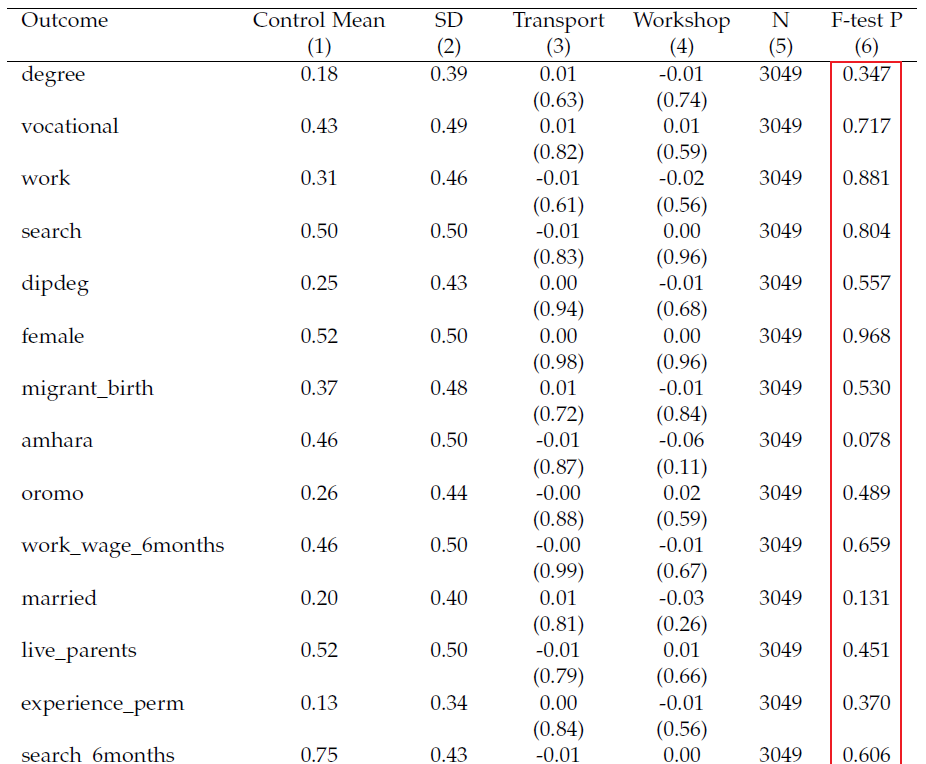
\includegraphics[width=5in]{images/ch6/Abebe balancing.png}
                \caption{Summary and Tests of Balance}
            \end{figure}
            If the samples are unbalanced, we should at least control for unbalanced variables later.
            
        \subsubsection{Data Collection}
            A combination of face-to-face interviews and phone follow ups. The \emph{attrition rate is very low}:
            \begin{figure}[H]
                \centering
                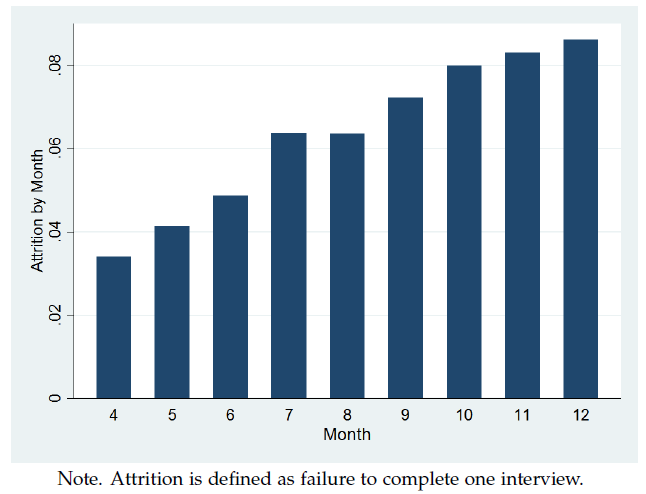
\includegraphics[width=4in]{images/ch6/Abebe attrition.png}
                \caption{Attrition Rate from the Phone Survey by Month}
            \end{figure}

    \subsection{Estimation}
    
        \subsubsection{Pre-Analysis Plan}
            The authors follow \emphb{a detailed pre-analysis plan} that describes the empirical strategy, outcome variables, subgroup analysis, etc.\par
            \textit{For RCTs, pre-analysis plans are typically important: they mitigate the possibility of ex post data snooping. Their effectiveness can be illustrated in this figure:}
            \begin{figure}[H]
                \centering
                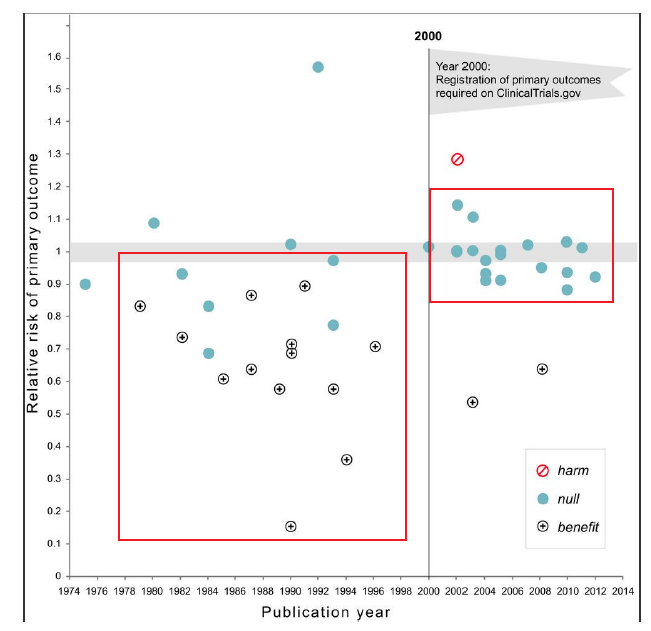
\includegraphics[width=4in]{images/ch6/pre-analsis plan and data snooping.png}
                \caption{Less Significant Results after Requiring Pre-Analysis Plan}
            \end{figure}
            \textit{The number of researches which claim the effectiveness of a drug decreased dramatically after the requirement of a pre-analysis plan.}
            
        \subsubsection{Main Regression}
            \begin{equation*}
                y_{ic} = \beta_0 + \sum_{f} \big[ \beta_f \text{treatment}_{fic} + \gamma_f \text{spillover}_{fic} \big] + \alpha y_{ic, pre} + \delta x_{ic0} + \mu_{ic}
            \end{equation*}
            where:
            \begin{itemize}
                \item $\text{treatment}_{fic}$: treatment dummy = 1 if an individual was offered treatment f
                \item $\text{spillover}_{fic}$: spillover dummy = 1 if an individual resided in a treated cluster
                \item $x_{ic0}$: baseline covariates used for re-randomisation and blocking (and to improve precision)
            \end{itemize}
            This regression can capture the \emph{intention-to-treat (ITT)} parameter, and we cluster standard errors at the geographical clusers level.
            
    \subsection{Results}
    
        \subsubsection{Overall Effect}
            \begin{figure}[H]
                \centering
                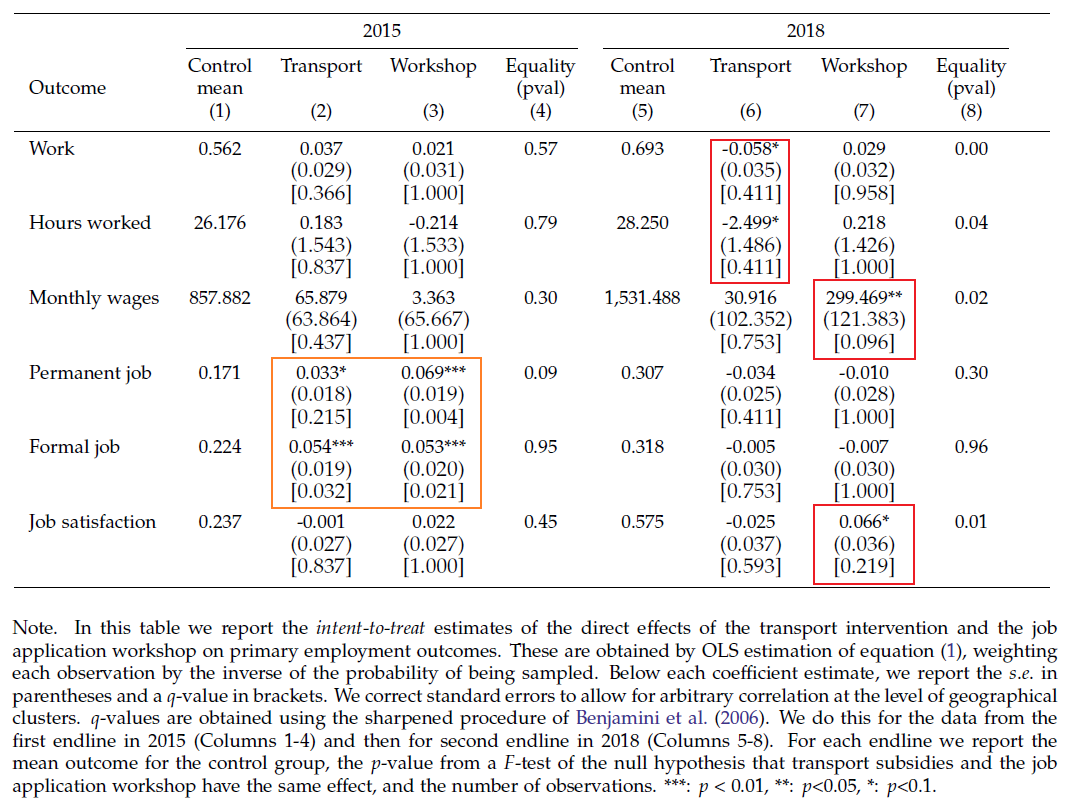
\includegraphics[width=5in]{images/ch6/Abebe result 1.png}
                \caption{ITT Estimates}
            \end{figure}
            Soon after the interventions (2015), significant positive effects are found on participants' rate of entering permanent jobs and formal jobs (orange square). However, 3 years later (2018), significant positive effects are only found for workshops (on monthly wages and job satisfaction). In contrast, transport subsidy is estimated to have significant negative effects on employment and hours worked.
            
        \subsubsection{Impact Trajectories: Employment and Permanent Employment}
            \begin{figure}[H]
                \centering
                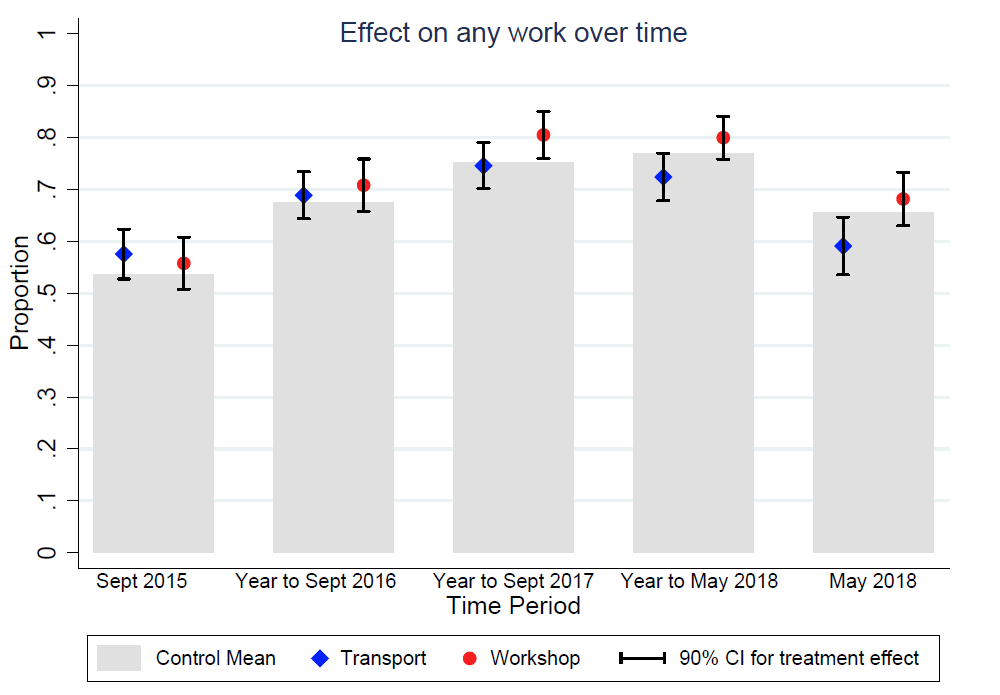
\includegraphics[width=2.75in]{images/ch6/Abebe result 2 emp.png}
                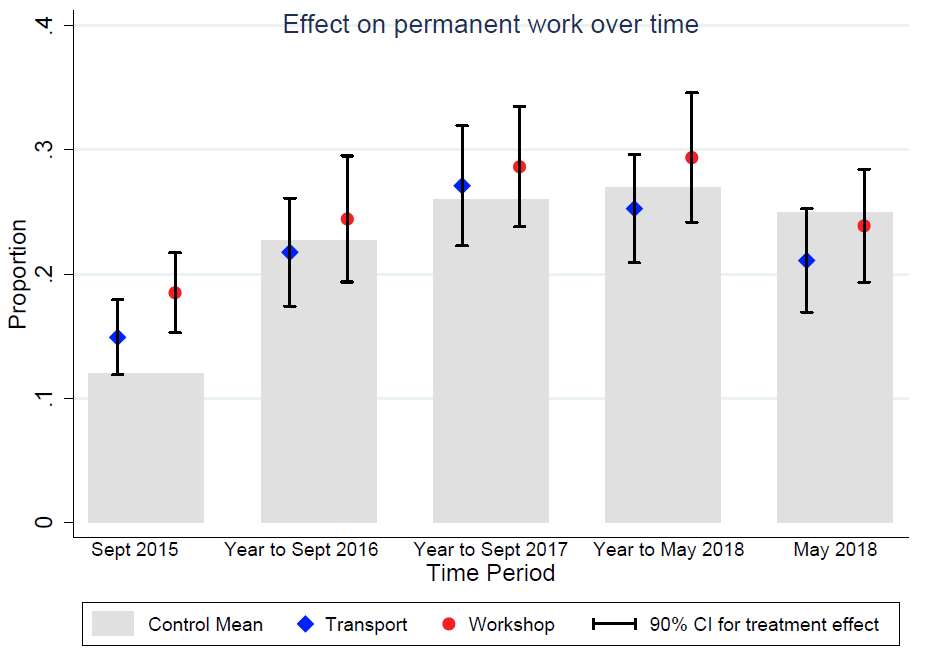
\includegraphics[width=2.75in]{images/ch6/Abebe result 2 perm emp.png}
                \caption{Impact Trajectories: Employment and Permanent Employment}
            \end{figure}
            No significant positive effects are found regarding employment or formal employment in the long term. However, transport subsidy negatively influences employment 4 years after the treatment.
            
        \subsubsection{Search Effort}
            \begin{figure}[H]
                \centering
                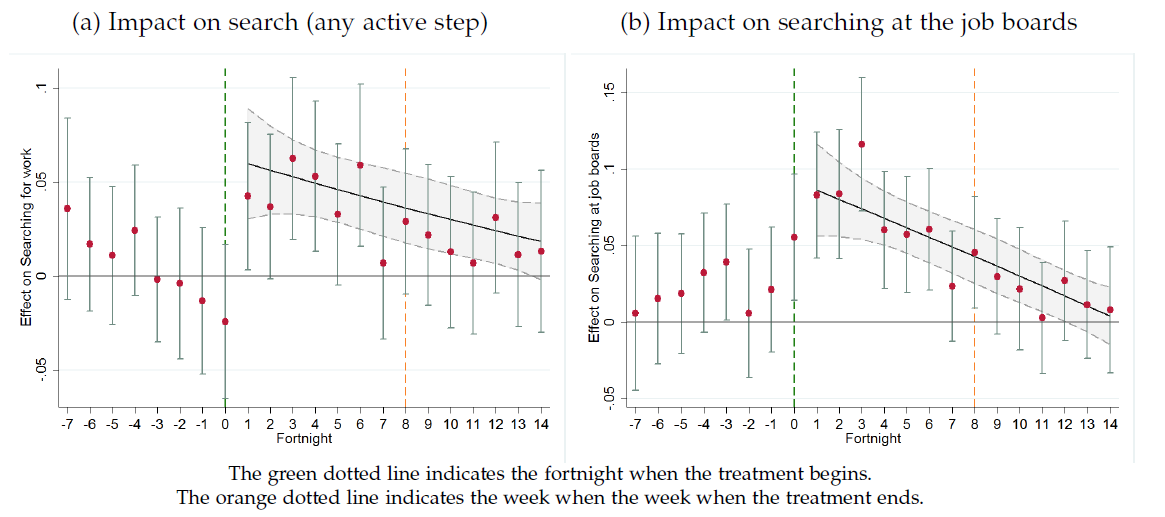
\includegraphics[width=5.5in]{images/ch6/Abebe result 3 search effort transport.png}
                \caption{Fortnightly Impacts of the Transport Treatment on Job Search}
            \end{figure}
            Transport subsidy facilitates job searching immediately after treatment, but such effect vanishes quickly: after 14 days, it becomes insignificant.
            \begin{figure}[H]
                \centering
                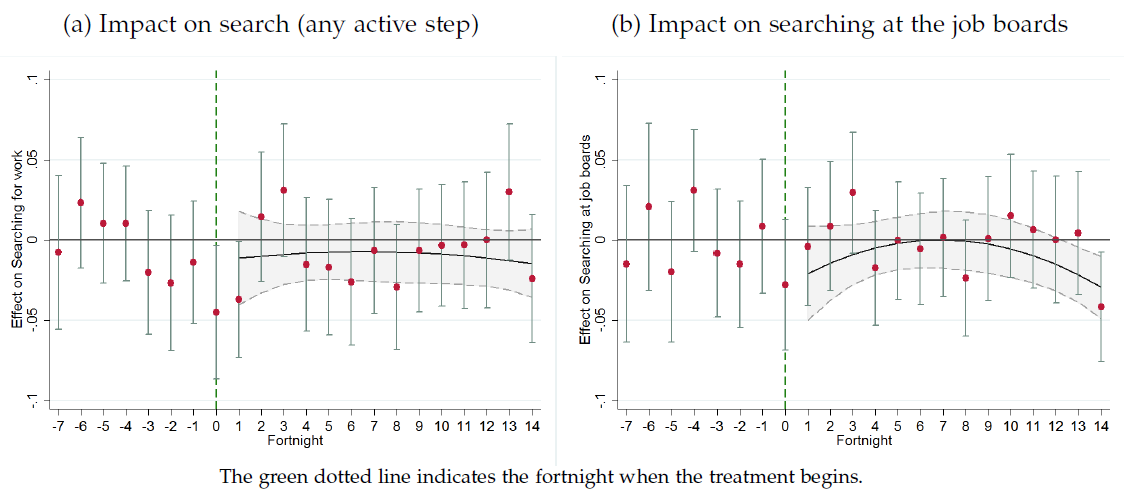
\includegraphics[width=5.5in]{images/ch6/Abebe result 3 search effort workshop.png}
                \caption{Fortnightly Impacts of the Job Application Workshop on Job Search}
            \end{figure}
            On the other hand, job application workshop has no effect on job search intensity at all. This indicates that the benefits brought by workshops are likely to be caused by better information efficiency between employers and job-seekers.
            
        \subsubsection{Match Quality}
            \begin{figure}[H]
                \centering
                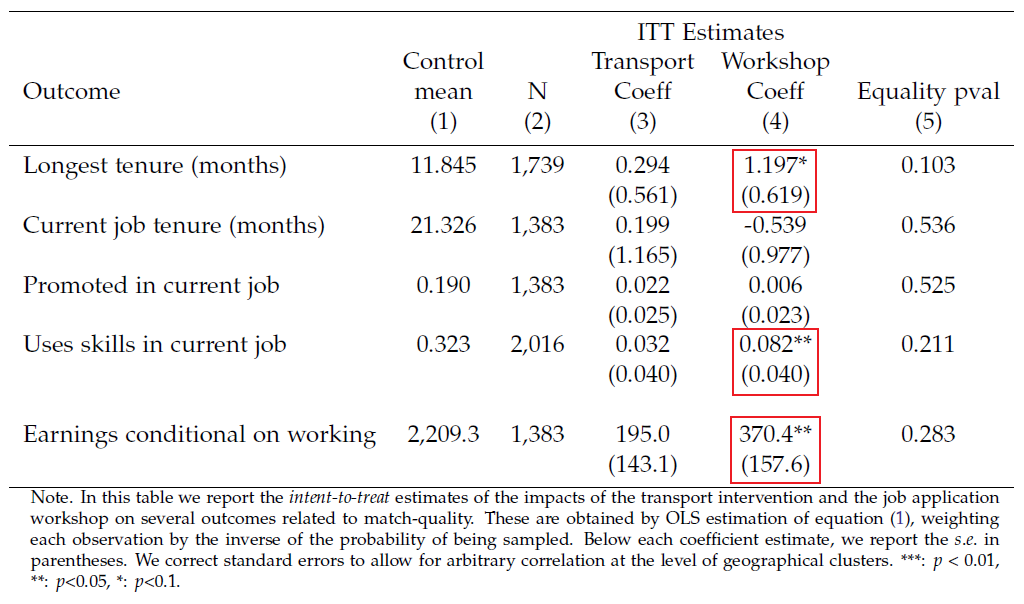
\includegraphics[width=4.5in]{images/ch6/Abebe result 4 matching quality.png}
                \caption{Impacts on Job Tenure and Conditional Earnings}
            \end{figure}
            After intervention, workshop treatment shows evidences of improvement in several job matching quality indicators (longest tenure, uses skills in current job, and earnings conditional on working). On the other hand, no significant effects are found for transport subsidy treatment.
            
        \subsubsection{Workshop Compared with Other Interventions}
            \begin{figure}[H]
                \centering
                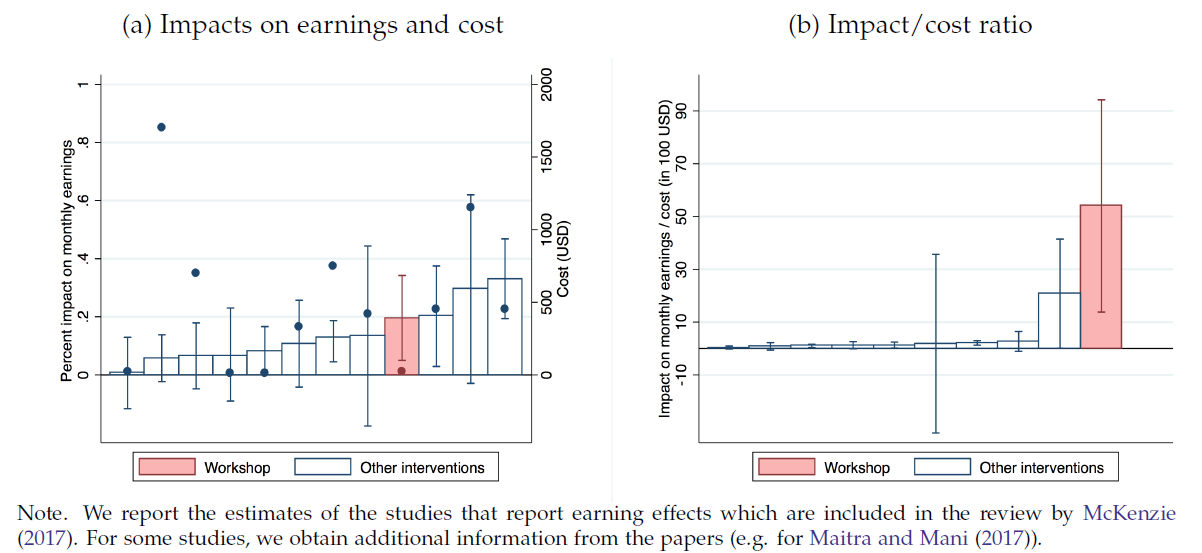
\includegraphics[width=5.5in]{images/ch6/Abebe result 5 compare with other policies.png}
                \caption{Comparison with Other ALMPs in Developing Countries}
            \end{figure}
            Compared with other interventions, job application workshops have significant positive effects on participants' monthly wages with low implementation costs, which endorse it with the \empha{highest impact/cost ratio} among all policies.
            
        \subsubsection{Heterogeneous Effects}
            \begin{figure}[H]
                \centering
                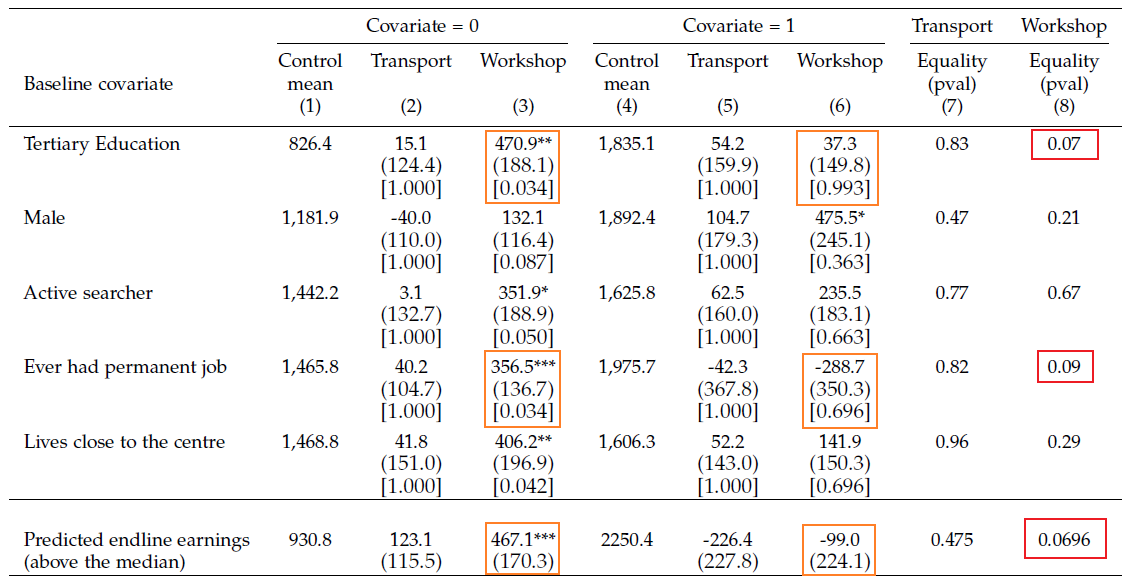
\includegraphics[width=5.5in]{images/ch6/Abebe result 6 heterogeneous.png}
                \caption{Heterogeneous Effects on 2018 Wage Earnings by Baseline Characteristics}
            \end{figure}
            Treatment effects are heterogeneous within the sample population. In the figure above, the column named "Covariate = 0" indicates the subsample whose baseline covariate (each row) = 0. For example, the orange square on row 1 column 3 indicates the estimated ITT of workshop on an individual without tertiary education.\par
            We can see that while there's no heterogeneity in ITT of transport subsidy (since it is ineffective for everyone...), obvious heterogeneity can be observed in the ITT of job application workshop: disadvantageous participants (with no tertiary education, did not ever have a permanent job, or with predicted endline earnings below median) are more likely to benefit from workshops.
            